\documentclass[a4paper,11pt]{beamer}

\mode<presentation> {

% The Beamer class comes with a number of default slide themes
% which change the colors and layouts of slides. Below this is a list
% of all the themes, uncomment each in turn to see what they look like.

%\usetheme{default}
%\usetheme{AnnArbor}
%\usetheme{Antibes}
%\usetheme{Bergen}
%\usetheme{Berkeley}
%\usetheme{Berlin}
%\usetheme{Boadilla}
%\usetheme{CambridgeUS}
%\usetheme{Copenhagen}
%\usetheme{Darmstadt}
%\usetheme{Dresden}
%\usetheme{Frankfurt}
%\usetheme{Goettingen}
%\usetheme{Hannover}
%\usetheme{Ilmenau}
%\usetheme{JuanLesPins}
%\usetheme{Luebeck}
\usetheme{Madrid}
%\usetheme{Malmoe}
%\usetheme{Marburg}
%\usetheme{Montpellier}
%\usetheme{PaloAlto}
%\usetheme{Pittsburgh}
%\usetheme{Rochester}
%\usetheme{Singapore}
%\usetheme{Szeged}
%\usetheme{Warsaw}

% As well as themes, the Beamer class has a number of color themes
% for any slide theme. Uncomment each of these in turn to see how it
% changes the colors of your current slide theme.

%\usecolortheme{albatross}
%\usecolortheme{beaver}
%\usecolortheme{beetle}
%\usecolortheme{crane}
%\usecolortheme{dolphin}
%\usecolortheme{dove}
%\usecolortheme{fly}
%\usecolortheme{lily}
%\usecolortheme{orchid}
%\usecolortheme{rose}
%\usecolortheme{seagull}
%\usecolortheme{seahorse}
%\usecolortheme{whale}
%\usecolortheme{wolverine}

%\setbeamertemplate{footline} % To remove the footer line in all slides uncomment this line
%\setbeamertemplate{footline}[page number] % To replace the footer line in all slides with a simple slide count uncomment this line

%\setbeamertemplate{navigation symbols}{} % To remove the navigation symbols from the bottom of all slides uncomment this line
}

\usepackage[absolute,overlay]{textpos}
%----------------------------
\usepackage[utf8]{inputenc}
\usepackage[spanish]{babel}
\usepackage[T1]{fontenc}
%----------------------------
\usepackage{graphicx}
\usepackage{booktabs}
\uselanguage{spanish}
\deftranslation[to=spanish]{Theorem}{Teorema}
\deftranslation[to=spanish]{theorem}{teorema}
\deftranslation[to=spanish]{Lemma}{Lema}
\deftranslation[to=spanish]{lemma}{lema}

\newcounter{saveenumi}
\newcommand{\seti}{\setcounter{saveenumi}{\value{enumi}}}
\newcommand{\conti}{\setcounter{enumi}{\value{saveenumi}}}

% \usepackage[toc]{glossaries} %xindy
% \makeglossaries
%----------------------------
\graphicspath{{imgs/}}

\title[ISDB-Tb Extendido]{Integración de servicios audiovisuales de TV terrestre e IPTV} % The short title appears at the bottom of every slide, the full title is only on the title page

\author{Santiago Seifert} % Your name
\institute[UNLP] % Your institution as it will appear on the bottom of every slide, may be shorthand to save space
{
Universidad Nacional de La Plata \\ % Your institution for the title page
\medskip
\textit{santiagoseifert@gmail.com} % Your email address
}
\date{\today} % Date, can be changed to a custom date

\begin{document}

\begin{frame}
\titlepage % Print the title page as the first slide
\end{frame}

% \begin{frame}
% \frametitle{Contenidos de la presentación} % Table of contents slide, comment this block out to remove it
% \tableofcontents % Throughout your presentation, if you choose to use \section{} and \subsection{} commands, these will automatically be printed on this slide as an overview of your presentation
% \end{frame}

% %----------------------------------------------------------------------------------------
% %  & PRESENTATION SLIDES
% %----------------------------------------------------------------------------------------

% %------------------------------------------------
% \section{First Section} % Sections can be created in order to organize your presentation into discrete blocks, all sections and subsections are automatically printed in the table of contents as an overview of the talk
% %------------------------------------------------

% \subsection{Subsection Example} % A subsection can be created just before a set of slides with a common theme to further break down your presentation into chunks


%------------------------------------------------
% TEMARIO.

\begin{frame}
	\frametitle{Temario}
	\tableofcontents
\end{frame}

\begin{frame}
\frametitle{Temario}
\begin{center}
\begin{itemize}
\item Introducción
	\begin{itemize}
		\item Motivación
		\item Hipótesis
		\item Objetivos
	\end{itemize}
\item Introducción Técnica
	\begin{itemize}
		\item Conceptos útiles
		\item ISDB-Tb
		\item Generación de contenidos en ISDB-Tb
		\begin{itemize}
			\item OpenCaster
		\end{itemize}
		\item Recepción y decodificación de contenidos en ISDB-Tb
		\begin{itemize}
			\item Reproductor de TV Digital \textbf{Wari}
		\end{itemize}
		\item IPTV
	\end{itemize}
\item Diseño y desarrollo
	\begin{itemize}
		\item Señalización
			\begin{itemize}
				\item Elementary Streams Relocation Descriptor
			\end{itemize}
		\item Construcción del Flujo de Transporte de referencia
			\begin{itemize}
				\item Extensión de OpenCaster
				\item Aumento de un Flujo de Transporte existente
			\end{itemize}
		\item Emisión de IPTV
		\item Recepción de Contenidos
			\begin{itemize}
				\item Reproductor de TV Híbrida \textbf{Mara}
			\end{itemize}
	\end{itemize}
\item Evaluación
	\begin{itemize}
		\item Infraestructura
			\begin{itemize}
				\item Escenario Real
				\item Escenario de prueba
			\end{itemize}
		\item Análisis General
			\begin{itemize}
				\item Número de Servicios
				\item Flujos Elementales Múltiples
				\item Guía electrónica de programación
				\item \emph{Closed Caption}
				\item Gestión de Audiencias
				\item Aplicaciones Interactivas
				\item Tiempos de sintonización
			\end{itemize}
	\end{itemize}
\item Conclusión
	\begin{itemize}
		\item Características del resultado
		\item Mara
		\item Trabajo Futuro
		\begin{itemize}
			\item Reubicación en \emph{Object Based Broadcasting}
			\item Reubicación por eventos
			\item Soporte de IPV6
			\item Omisión de PMT pequeñas
		\end{itemize}
		\item Conclusión
	\end{itemize}
\end{itemize}

\end{center}
\end{frame}


%------------------------------------------------

\begin{frame}
\frametitle{ISDB-T}
\begin{center}
\begin{itemize}
\item Broadcast por radiofrecuencia
\item Ancho de banda limitado
\item Canales de 6Mhz
\end{itemize}

\includegraphics[width=4cm]{antenna.png}
\end{center}
\end{frame}

%------------------------------------------------

\begin{frame}
\frametitle{ISDB-T}
\begin{center}
\begin{figure}
  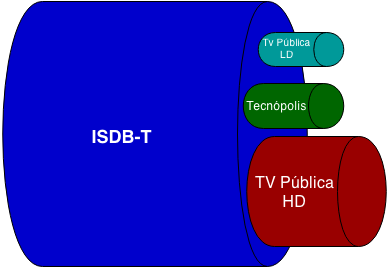
\includegraphics[width=6cm]{isdbtcable_regular.png} \caption{Canal 23 (527Mhz), de Junio}
\end{figure}
\end{center}
\end{frame}

%------------------------------------------------

\begin{frame}
\frametitle{ISDB-T}
\begin{center}
\begin{figure}
 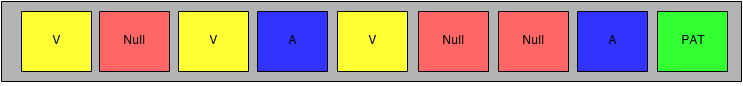
\includegraphics[width=11cm]{ts.png} \caption{Formato contenedor utilizado en ISDB-T: \textbf{MPEG-TS}}
\end{figure}
\end{center}
\end{frame}

%------------------------------------------------

\begin{frame}
\frametitle{ISDB-T}
\begin{center}
\begin{figure}
 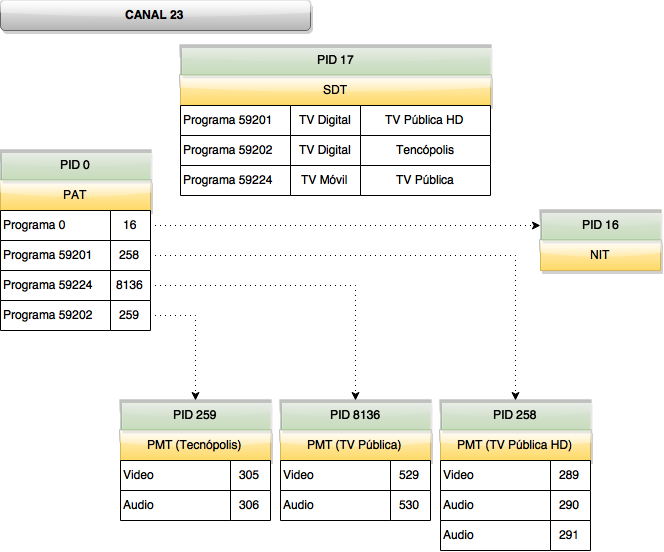
\includegraphics[height=6.5cm]{canal_23_tables.png} \caption{Tablas del \textbf{MPEG-TS}}
\end{figure}
\end{center}
\end{frame}

%------------------------------------------------

\begin{frame}
\frametitle{IPTV}
\begin{center}
\textbf{Definición de ITU:} IPTV define a la entrega de servicios como televisión/video/audio/texto/imágenes/datos sobre redes basadas en IP manejadas para proveer el nivel requerido de calidad de servicio y experiencia, seguridad, interactividad y confiabilidad.

\only<1>{
\begin{figure}
 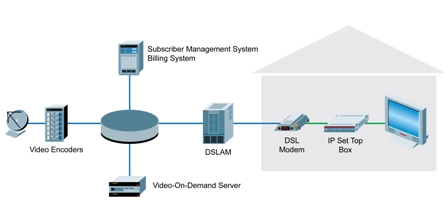
\includegraphics[width=8cm]{iptv.jpg}
\end{figure}
}

\only<2>{
\begin{figure}
 
\includegraphics[height=3cm]{deal_with_it.jpg}
\end{figure}
}
\end{center}
\end{frame}

%------------------------------------------------

\begin{frame}
\frametitle{IPTV - Multicast}
\begin{figure}
 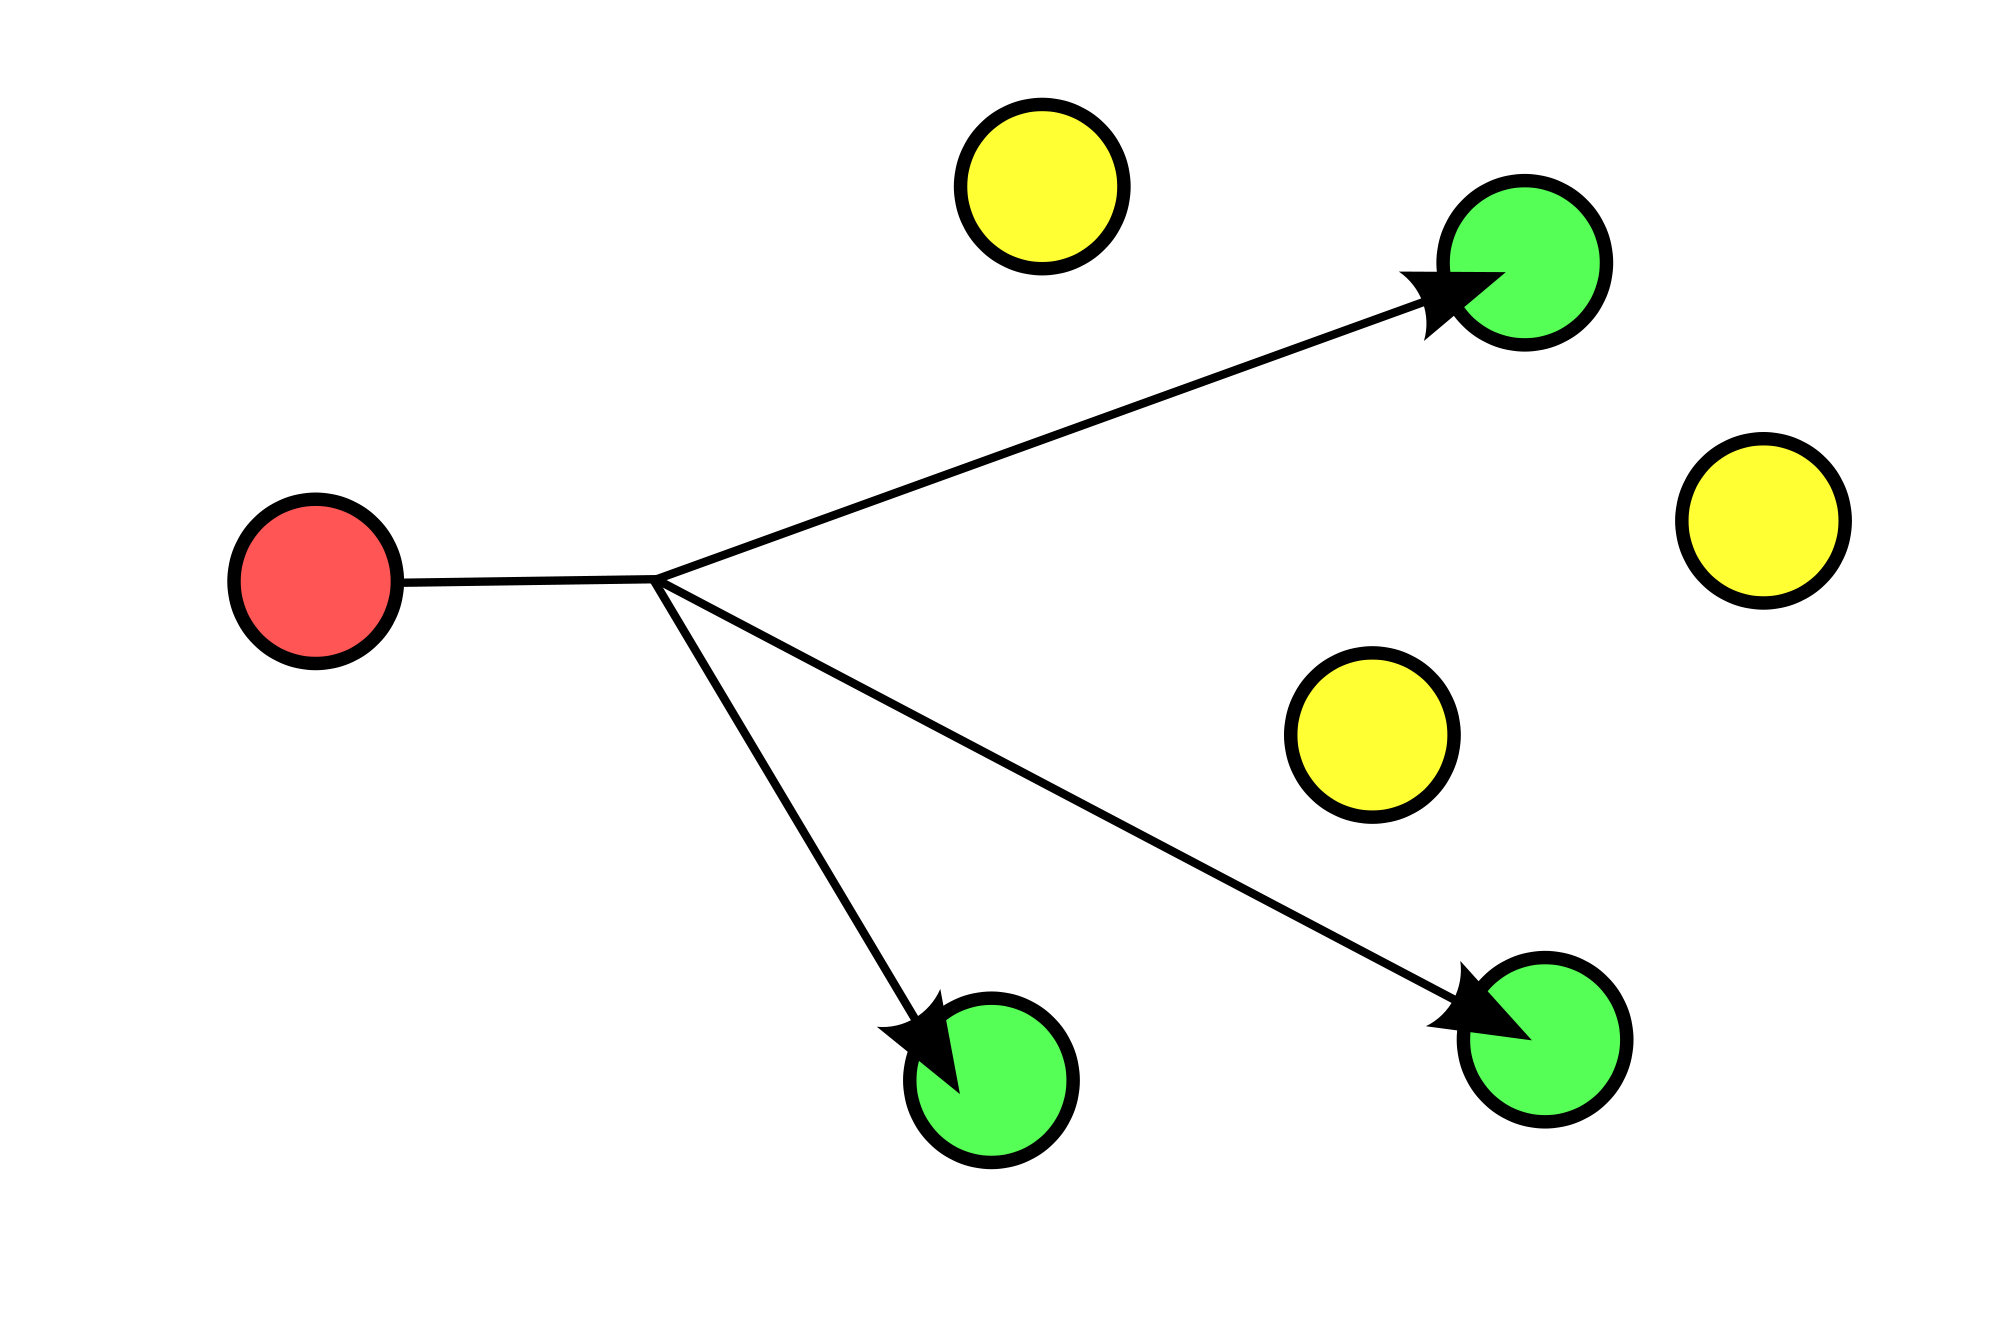
\includegraphics[height=7cm]{multicast.png}
\end{figure}
\end{frame}

%------------------------------------------------


\begin{frame}
\frametitle{IPTV - Multicast}
\begin{figure}
 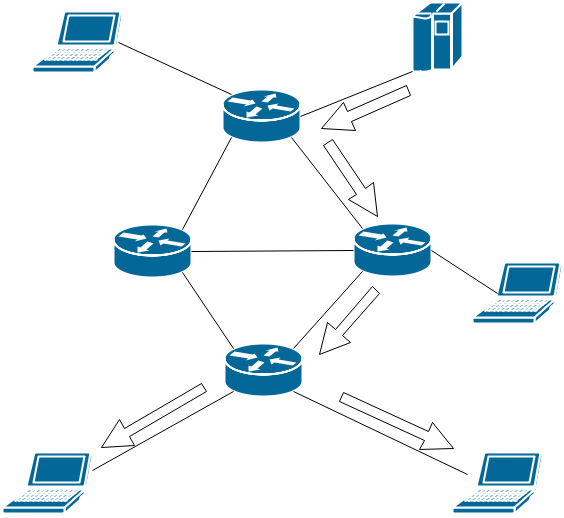
\includegraphics[height=7cm]{topoloy.png}
\end{figure}
\end{frame}

%------------------------------------------------


\begin{frame}
\frametitle{Comparación}
\begin{columns}[c,t] % The "c" option specifies centered vertical alignment while the "t" option is used for top vertical alignment

\column{.45\textwidth} % Left column and width
\textbf{ISDB-T}
\begin{enumerate}
\item Robusto
\item Limitación de servicios
\item Infraestructura simple
\end{enumerate}

\column{.45\textwidth} % Right column and width
\textbf{IPTV}
\begin{enumerate}
\item Suceptible a sobreexigencia
\item Lista de servicios potencialmente grande
\item Infraestructura compleja
\end{enumerate}
\end{columns}
\end{frame}

%------------------------------------------------
%------------------------------------------------

\begin{frame}
\frametitle{Problema actual}
\framesubtitle{No está la telenovela ``La gata'' de la nona, en canal de las estrellas}
\begin{center}
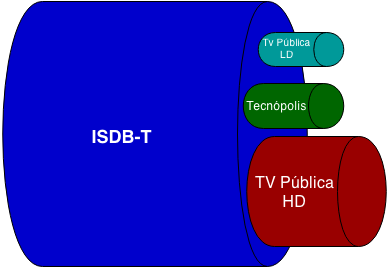
\includegraphics[width=7cm]{isdbtcable_regular.png}
\end{center}
\end{frame}

%------------------------------------------------

\begin{frame}
\frametitle{Definiciones (Problema y motivación)}
\begin{lemma}[de la turba iracunda]
Si el partido de Boca-River se corta, la turba sale a matar \emph{nerds}.
\end{lemma}
\begin{lemma}[de la nona iracunda]
Si la nona no ve la novela, no hay tallarines, y sale a matar \emph{nerds}.
\end{lemma}
\begin{lemma}[del nerd muerto]
Un nerd muerto no puede jugar a la computadora, comer comida y mirar \emph{9gag}.
\end{lemma}
\end{frame}


%------------------------------------------------

\begin{frame}
\frametitle{Aspectos de la solución}


\begin{columns}[c] % The "c" option specifies centered vertical alignment while the "t" option is used for top vertical alignment

\column{.45\textwidth} % Left column and width
\begin{itemize}
\item Transmisión IP
\item Señalización ISDB-T
\item Reproducción
\end{itemize}


\column{.45\textwidth} % Right column and width
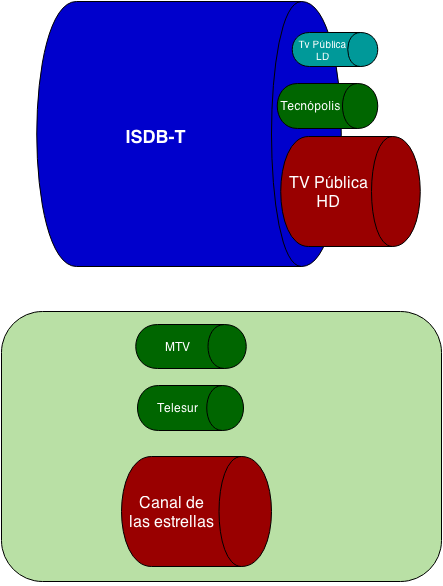
\includegraphics[height=7cm]{isdbtcable_extended.png}

\end{columns}

%\begin{figure}
%\end{figure}
\end{frame}



%------------------------------------------------

\begin{frame}
\frametitle{Transmisión IP}
Acá hay que desarrollar los siguientes conceptos:
\begin{itemize}
\item Televisión en vivo -> Multicast
\item Multicast -> UDP
\item UDP -> MPEG-TS
\end{itemize}
\end{frame}


%------------------------------------------------

\begin{frame}
\frametitle{Transmsión ISDB-T}
\begin{center}
\begin{figure}
 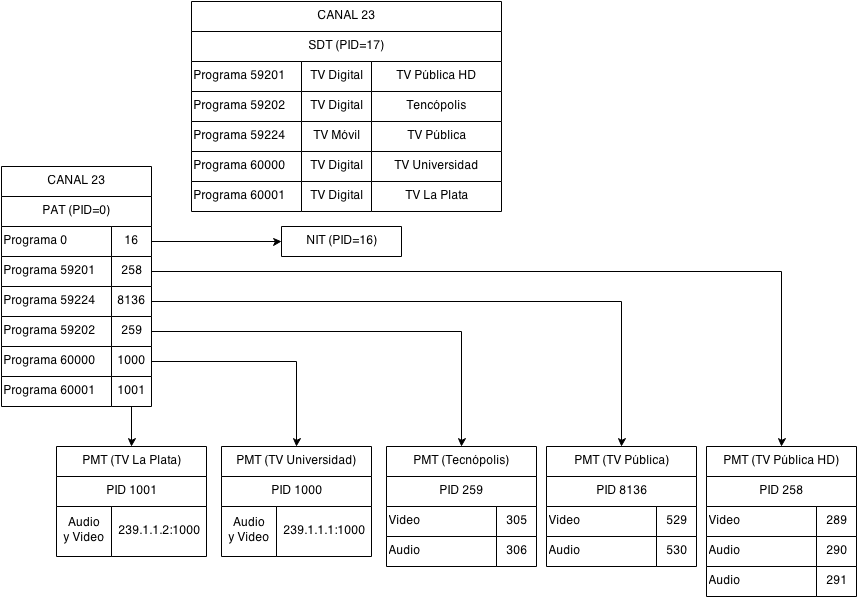
\includegraphics[height=6.5cm]{canal_23_extended_tables.png} \caption{Tablas del \textbf{MPEG-TS}}
\end{figure}
\end{center}
\end{frame}

%------------------------------------------------

\begin{frame}
\frametitle{Sintaxis PMT - Parte 1}
\begin{tabular}{ l | c | c }
syntax & bit index & \# of bits \\
\hline 
table\_id & 0 & 8 \\
section\_syntax\_indicator & 8 & 1 \\
``0'' & 9 & 1 \\
reserved & 10 & 2 \\
section\_length & 12 & 12 \\
program\_number & 24 & 16 \\
reserved & 40 & 2 \\
version\_number & 42 & 5 \\
current\_next\_indicator & 47 & 1 \\
section\_number & 48 & 8 \\
last\_section\_number & 56 & 8 \\
reserved & 64 & 3 \\
PCR\_PID & 67 & 13 \\
\end{tabular}
\end{frame}

%------------------------------------------------

\begin{frame}
\frametitle{Sintaxis PMT - Parte 2}
\begin{tabular}{ l | c | c }
syntax & bit index & \# of bits \\
\hline 
reserved  & 80  & 4\\
program\_info\_length  & 84  & 12\\
descriptor()  & 96  & varA \\
for i = 0 to N \{& - & -\\
  \ \ \ stream\_type  & 96 + varA  & 8 \\
  \ \ \ reserved  & 104 + varA  & 3 \\
  \ \ \ elementary\_PID  & 107 + varA  & 13 \\
  \ \ \ reserved  & 120 + varA & 4 \\
  \ \ \ ES\_info\_length  & 124 + varA & 12 \\
  \ \ \ descriptor()  & 136 + varA  & varA  \\
\} & - & - \\
CRC\_32  & - & 32 \\
\end{tabular}
\end{frame}

%------------------------------------------------

\begin{frame}
\frametitle{Elementaries relocation descriptor}
\begin{tabular}{ l | c | c }
syntax & bit index & \# of bits \\
\hline 
descriptor\_length(``6'')  & 0  & 8 \\
multicast\_group\_ip  & 8  & 32\\
multicast\_group\_port  & 40 & 16 \\

\end{tabular}
\end{frame}

%------------------------------------------------
\begin{frame}
\frametitle{Software de recepción y reproducción - Parte 1}
\textbf{Pasos en el mecanismo de selección de programas:}
\begin{enumerate}
\item Scan, memorizando tablas de \emph{System information} (NIT, SDT, etc), y armar lista de servicios
\item Sintonizar el canal asociado al servicio seleccionado y sincronizarse
\item Filtrar PAT y de ella extraer el PID de la PMT asociada
\item Filtrar PMT y extraer PIDs de flujos elementales y PCR (asumiendo que no hay acceso condicional). \textbf{Para servicios reubicados, los paquetes se obtienen de la dirección multicast obtenida por el descriptor.}
\seti
\end{enumerate}
% \begin{textblock*}{2cm}(10cm,1cm) % {block width} (coords)
% 
\includegraphics[width=1cm]{synchronized1.png}
% \end{textblock*}
\end{frame}

%------------------------------------------------

\begin{frame}
\frametitle{Software de recepción y reproducción - Parte 2}
\textbf{Pasos en el mecanismo de selección de programas:}
\begin{enumerate}
\conti
\item En base al listado de PIDs, filtrar paquetes de flujos elementales
\item Reconstruir paquetes PES, y luego los flujos elementales ES
\item Decodificación y reproducción
\end{enumerate}
\end{frame}

%------------------------------------------------

\begin{frame}
\frametitle{Software de recepción: Proyecto Kuntur}
\begin{itemize}
\item Código abierto
\item Desarrollado por el LIFIA, dependiente de la facultad de informática de UNLP
\item Posee una librería reutilizable llamada \texttt{mpegparser}
\item Cualquier modificación se aplica a todos los reproductores del proyecto
\end{itemize}
\end{frame}

%------------------------------------------------

\begin{frame}
\frametitle{Kuntur: ¿Cuáles son los pasos para modificarlo?}
\begin{enumerate}
\item Agregar un modelo del descriptor
\item Identificar el descriptor en la PMT
\item Identificar al servicio como \emph{relocated}
\item Guardar referencia al grupo multicast y al puerto\\
\hrulefill
\item Una vez el usuario sintoniza el servicio, \emph{sacar los flujos elementales de internet}
\end{enumerate}
\end{frame}

%------------------------------------------------

\begin{frame}
\frametitle{Pruebas a realizar}
Acá hay que desarrollar los siguientes conceptos:
\begin{itemize}
\item Un ts con 15 servicios, por ejemplo. No hace falta emitirlos a todos, si no que apunten al mismo
\item Un ts con 2 servicios, cada uno con un grupo multicast distinto
\item Un ts con 2 servicios, uno con grupo multicast sin emisión
\item Dos ts con un servicio IPTV cada uno.
\end{itemize}
\end{frame}

%------------------------------------------------
\begin{frame}
\frametitle{Resultados esperados}
A desarrollar

Un ts con 15 servicios, por ejemplo. No hace falta emitirlos a todos, si no que apunten al mismo
Puede darse sobrecarga en el receptor? No debería. La lista de servicios sería anormalmente grande.
\end{frame}

%------------------------------------------------
\begin{frame}
\frametitle{Resultados esperados}
A desarrollar

Un ts con 2 servicios, cada uno con un grupo multicast distinto
No hay mucho lugar a la interpretación. Debería andar bien.
\end{frame}

%------------------------------------------------
\begin{frame}
\frametitle{Resultados esperados}
A desarrollar

Un ts con 2 servicios, uno con grupo multicast sin emisión
El que no tiene emisión debería quedarse sin reproducir nada. Pero no debería romper al receptor.
\end{frame}


%------------------------------------------------

\begin{frame}
\frametitle{Pruebas locas a realizar}
Acá hay que desarrollar los siguientes conceptos:
\begin{itemize}
\item Realizar la gestión por eventos y \emph{rating}

\end{itemize}
\end{frame}

%------------------------------------------------

\begin{frame}
\frametitle{Conclusión}
\begin{itemize}
\item Integra ISDB-T e IPTV
\item Señalización centralizada aprovechando la infraestructura de MPEG-TS
\item Transparente para el usuario
\item Listas de servicios potencialmente enormes
\item Modificación mínima del software de recepción
\item Modificación mínima del formato MPEG-TS
\end{itemize}
\end{frame}

%------------------------------------------------

\begin{frame}
\Huge{\centerline{End of transmission}}
\end{frame}

%----------------------------------------------------------------------------------------

\end{document} 